จากการค้นคว้าหาเครื่องมือในการสร้างคำกำกับข้อมูลเพื่อใช้เป็นแนวทางในการออกเครื่องมือสำหรับกำกับข้อมูลด้วยปัญญาประดิษฐ์ พบเครื่องมือที่เปิดให้ใช้ง่นสาธารณะ (open source) 2 เครื่องมือ 
คือ DarkLabel และ OpenLabeling โดยสรุปข้อสำคัญได้ดังนี้ 
\subsubsection*{โปรแกรม DarkLabel}
เป็นโปรแกรมที่ช่วยในการทำนายคำกำกับและบันทึกในรูปแบบต่างๆ รองรับข้อมูลป้อนเข้าในรูปแบบไฟล์วิดีโอ avi, mpg หรือกลุ่มรูปภาพ มีขั้นตอนการสร้างคำกำกับดังนี้ 
\begin{enumerate}
	\setlength\itemsep{-0.25em}
	\item สร้างกรอบสี่เหลี่ยมครอบบริเวณวัตถุที่สนใจโดยใช้มนุษย์เป็นคนสร้าง
	\item กดปุ่ม Next และ Predict อย่างต่อเนื่อง เพื่อทำนายตำแหน่งต่อไปของกรอบสี่เหลี่ยมในเฟรมถัดๆไป จนกระทั่งการเกิดข้อผิดพลาด
	\item ลบกรอบสี่เหลี่ยมที่พลาด และเริ่มทำขั้นตอนที่ 1 ใหม่ อีกครั้งจนครบทุกเฟรมในวิดีโอ
\end{enumerate}
หลังจากที่ผู้วิจัยได้ทดลองใช้โปรแกรม DarkLabel พบว่า เป็นโปรแกรมที่การทำงานส่วนใหญ่เป็นการสร้างคำกำกับแบบใช้มนุษย์เป็นคนทำด้วยตัวเอง ซึ่งทำให้ใช้เวลาในการทำนาน

\begin{figure}[!ht]
	\centering
	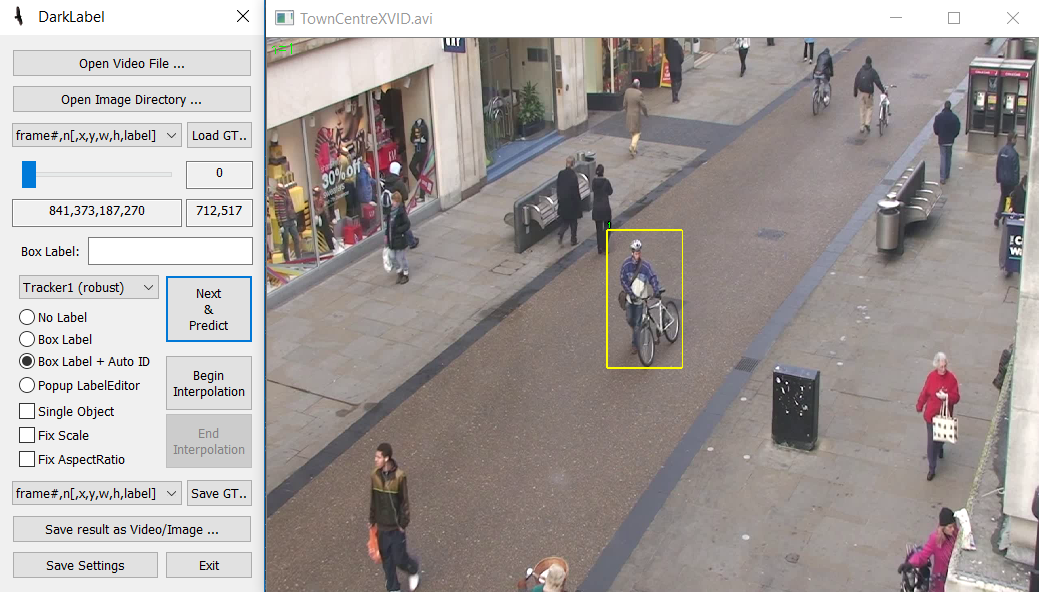
\includegraphics[width=0.7\textwidth]{chapter2/images/darklabel.png}
		\caption{UI ของโปรแกรม DarkLabel}
    	\label{fig:darklabel}
\end{figure}
\clearpage

\subsubsection*{โปรแกรม OpenLabeling}
เป็นโปรแกรมที่ช่วยในการทำนายคำกำกับ โดยโปรแกรมจะมีการทำงานอยู่ 2 รูปแบบการทำงาน คือแบบทำด้วยตัวเอง (Mode Manual) และแบบอัตโนมัติ (Mode Auto) ซึ่งมีการทำงานแยกจากกันอย่างชัดเจน 

\begin{enumerate}
	\setlength\itemsep{-0.25em}
	\item การทำงานแบบอัตโนมัติ 
	\\ หลังจากป้อนวิดีโอเข้าไปในโปรแกรมแล้วมีขั้นตอนการสร้างคำกำกับดังนี้ 
   	\begin{enumerate}
	\setlength\itemsep{-0.25em}
		\item โปรแกรมจะทำงานอัตโนมัติ โดยใช้โมเดลปัญญาประดิษฐ์ในการทำนายคีย์เฟรม (keyframe) 
		และทำนายตำแหน่งต่อไปของกรอบสี่เหลี่ยมในเฟรมถัดไปด้วยอัลกอริทึมที่ใช้การคำนวณคณิตศาสตร์และการประมวลผลภาพ (image processing) ในภาพที่เหลือ ผลลัพธ์ที่ได้คือรูปภาพและไฟล์ข้อมูลคำกำกับ
 	\end{enumerate}
	\item การทำงานแบบทำด้วยตัวเอง 
	\\ หลังจากป้อนวิดีโอเข้าไปในโปรแกรมแล้วมีขั้นตอนการสร้างคำกำกับดังนี้ 
	\begin{enumerate}
	\setlength\itemsep{-0.25em}
		\item สร้างกรอบสี่เหลี่ยมขึ้นมาโดยใช้มนุษย์เป็นคนสร้าง
		\item กดปุ่มเพื่อทำนายตำแหน่งต่อไปของกรอบสี่เหลี่ยมในเฟรมถัดไป จนกระทั่งเกิดข้อผิดพลาด
		\item ลบกรอบสี่เหลี่ยมที่พลาด และเริ่มทำขั้นตอนที่ 1 อีกครั้งจนครบทุกเฟรมในวิดีโอ
 	\end{enumerate}
 \end{enumerate}
หลังจากที่ได้ทดลองใช้โปรแกรม OpenLabeling ทั้ง 2 รูปแบบการทำงานแล้วพบว่า การทำงานแบบอัตโนมัติไม่สามารถปรับแก้ไขสิ่งใดในระหว่างกระบวนการนั้น 
ทำให้หากเกิดกรณีที่โมเดลทำนายกรอบสี่เหลี่ยมพลาดหรือเกินมา จะไม่สามารถแก้ไขได้ และการทำงานแบบทำด้วยตัวเองไม่มีระบบตรวจสอบกรอบสี่เหลี่ยม ทำให้ผู้ใช้งานจะต้องสร้างกรอบสี่เหลี่ยมขึ้นมาเอง

\begin{figure}[!ht]
	\centering
	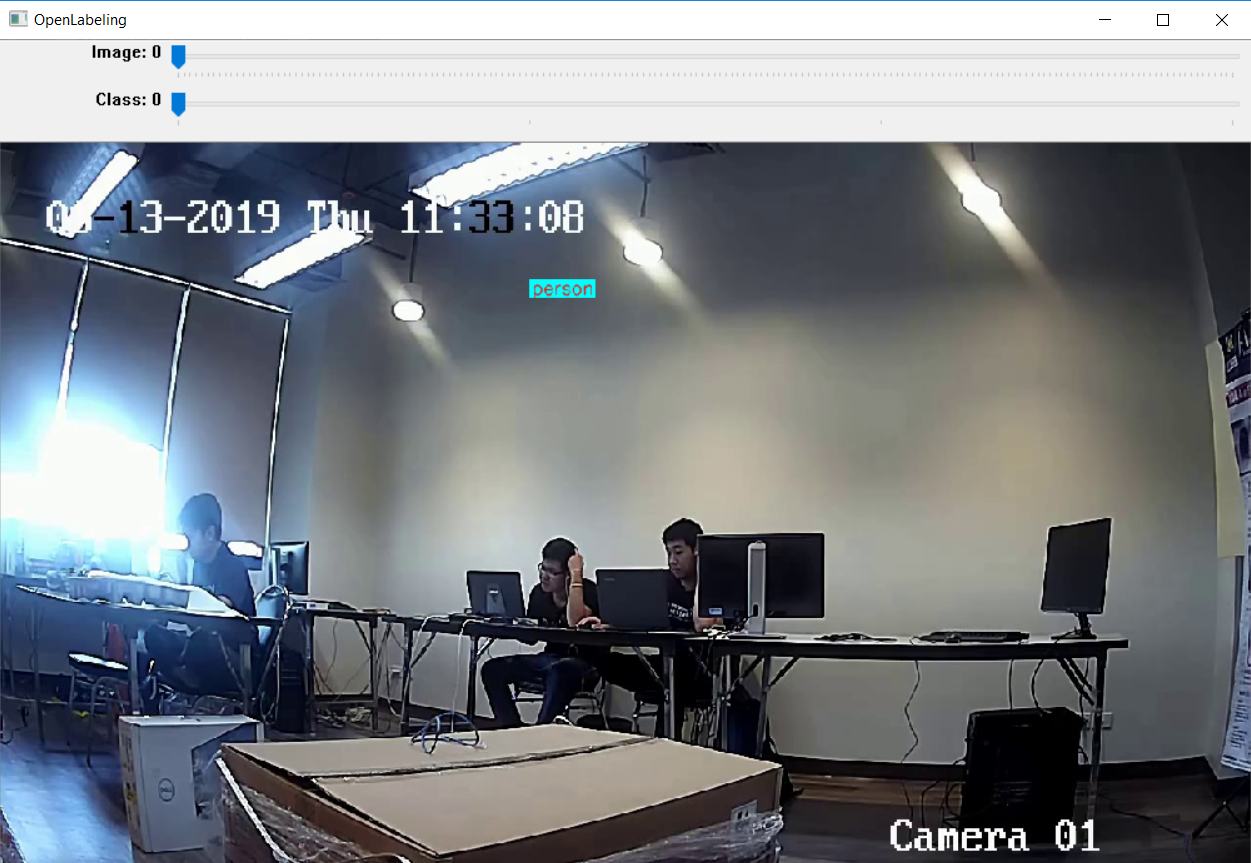
\includegraphics[width=0.7\textwidth]{chapter2/images/openlabel.png}
		\caption{UI ของโปรแกรม OpenLabeling}
    	\label{fig:openlabel}
\end{figure}


